\documentclass[journal,onecolumn]{IEEEtran}

% --- packages ---
\usepackage{graphicx}
\usepackage{tikz}
\usepackage{pgfplots}
\usepackage{float}            % [H] で強制配置
\usepackage{booktabs}
\usepackage{siunitx}
\usepackage{setspace}
\usepackage[margin=25mm]{geometry}

\pgfplotsset{compat=1.18}
\usetikzlibrary{arrows.meta,positioning}

% ---- title ----
\title{\LARGE Supplementary Figures and Tables for\\
\textit{``FeFET CMOS 0.18~$\mu$m Integration Study''}}
\author{}  % 別冊なので著者は省略
\date{}    % 日付非表示

\begin{document}
\maketitle
\thispagestyle{empty}

%========================================================
% Page 1 : Fig.1 + Table I  (中央寄せ、間隔広め)
%========================================================

% -------- Fig.1 : プロセス縦配置(中央寄せ) --------
\begin{figure}[H]\centering
% --- ダッシュ枠付きの縦フロー(例:最新TikZに差し替え可) ---
\begin{tikzpicture}[node distance=6mm,>=Stealth, every node/.style={font=\small}]
  \tikzset{step/.style={draw,rounded corners,minimum width=34mm,minimum height=5mm}}
  \node[step] (a) {Active / Isolation};
  \node[step,below=of a] (b) {VT Adjust / Well};
  \draw[->] (a)--(b);
  \node[step,below=of b] (c) {Poly Gate Definition};
  \draw[->] (b)--(c);
  \node[step,below=of c] (d) {LDD / Spacer};
  \draw[->] (c)--(d);
  \node[step,below=of d] (e) {Source/Drain Implant};
  \draw[->] (d)--(e);
  \node[step,below=of e] (f) {Salicide (Co)};
  \draw[->] (e)--(f);

  % --- FeFET 追加モジュール(点線囲み) ---
  \node[draw,dashed,rounded corners,minimum width=96mm,minimum height=21mm,
        below=14mm of f,anchor=north west] (box) {};
  \node[step,anchor=north west,xshift=4mm,yshift=-2mm] (g) at (box.north west)
      {FeFET Gate-Last: IL/FE/CAP (ALD) + TiN (PVD/ALD)};
  \node[step,below=of g] (h) {Crystallization RTA (\SI{450}{-}\SI{500}{\celsius}) + FGA (\SI{350}{\celsius})};
  \node[step,below=7mm of box.south] (i) {ILD + Vias + BEOL};
  \draw[->] (f) -- (box.north |- f.south);
  \draw[->] (box.south) -- (i);

  % 右側メモ
  \node[align=left,anchor=west] at ([xshift=6mm]box.east) {%
    Added mask: +1 (FE metal gate)\\
    FE anneal: BEOL furnace (no extra mask)\\
    TiN: long-throw / collimated sputter
  };
\end{tikzpicture}

\vspace{2mm}
\caption{Placement of the FeFET gate-last module within the 0.18~$\mu$m CMOS baseline (vertical layout).}
\label{fig:flow}
\end{figure}

% Fig.1 と Table の間隔(しっかり空ける)
\vspace{6mm}

% -------- Table I : 追加マスク(中央寄せ) --------
\begin{table}[H]\centering
\caption{Added masks / process steps relative to baseline logic.}
\label{tab:masks}
\begin{tabular}{@{}llp{74mm}@{}}
\toprule
\textbf{Step} & \textbf{Mask} & \textbf{Comment}\\
\midrule
FE metal gate & +1 & Reuse analog option route\\
FE anneal     & 0  & Performed in BEOL furnace (no extra mask)\\
\bottomrule
\end{tabular}
\end{table}

\clearpage
%========================================================
% Page 2 : Reliability data  Fig.2, Fig.3(top/bottom), Fig.4
%========================================================

% -------- Fig.2 : Endurance(中央寄せ・フル幅寄り) --------
\begin{figure}[H]\centering
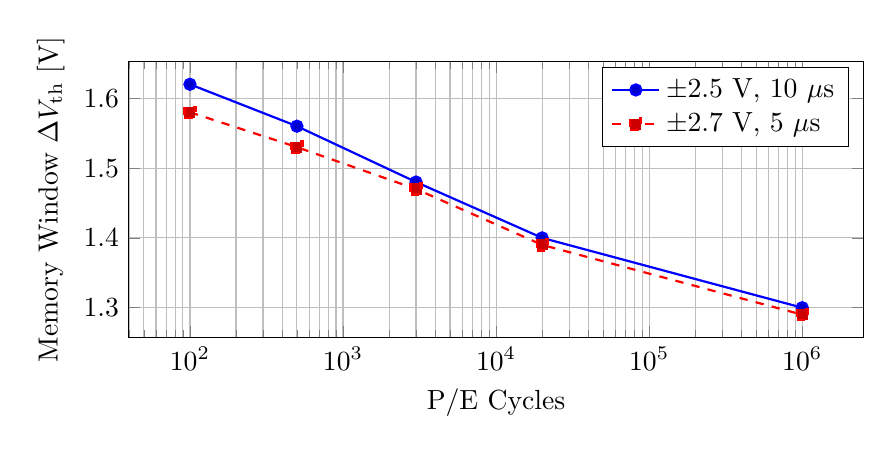
\begin{tikzpicture}
\begin{axis}[
  width=0.9\linewidth,height=0.42\linewidth,
  xlabel={P/E Cycles}, xmode=log, log basis x=10,
  ylabel={Memory Window $\Delta V_{\mathrm{th}}$ [V]},
  grid=both, legend columns=1, legend cell align=left]
\addplot+[mark=*,thick] coordinates {(1e2,1.62) (5e2,1.56) (3e3,1.48) (2e4,1.40) (1e6,1.30)};
\addlegendentry{$\pm 2.5$ V, 10 $\mu$s}
\addplot+[mark=square*, dashed,thick] coordinates {(1e2,1.58) (5e2,1.53) (3e3,1.47) (2e4,1.39) (1e6,1.29)};
\addlegendentry{$\pm 2.7$ V, 5 $\mu$s}
\end{axis}
\end{tikzpicture}
\caption{Schematic endurance behavior of HZO-FeFETs in a 0.18~$\mu$m flow.}
\label{fig:endurance}
\end{figure}

% -------- Fig.3 : Wake-up(上) + Retention(下) 縦並び・中央寄せ --------
\begin{figure}[H]\centering
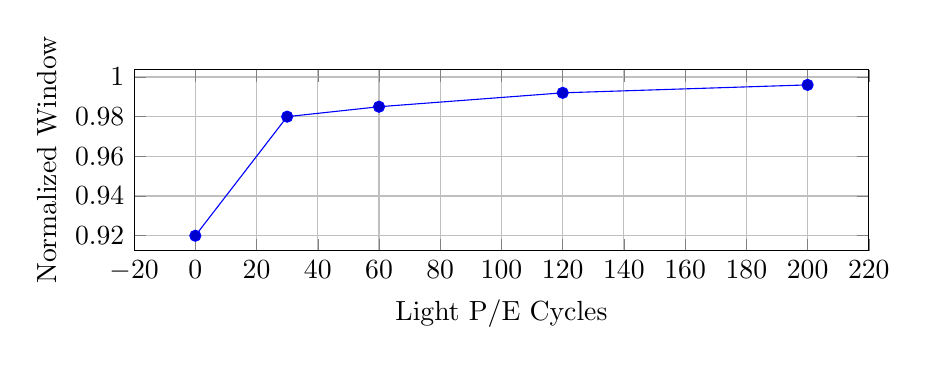
\begin{tikzpicture}
\begin{axis}[
  width=0.9\linewidth,height=0.32\linewidth,
  xlabel={Light P/E Cycles}, ylabel={Normalized Window},
  grid=both]
\addplot+[mark=*] coordinates {(0,0.92) (30,0.98) (60,0.985) (120,0.992) (200,0.996)};
\end{axis}
\end{tikzpicture}

\vspace{2mm}

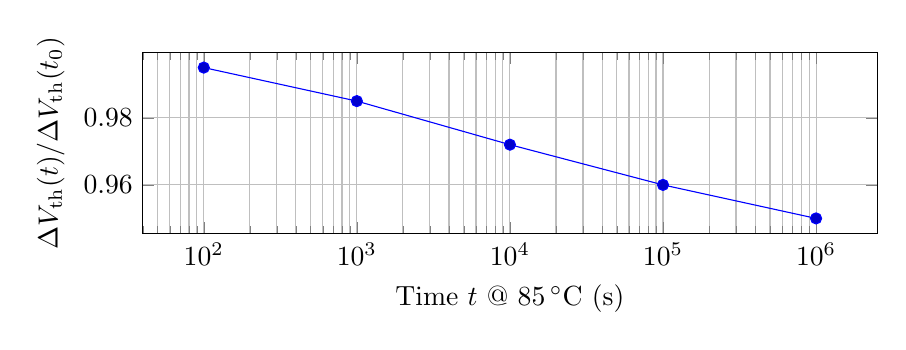
\begin{tikzpicture}
\begin{axis}[
  width=0.9\linewidth,height=0.32\linewidth,
  xmode=log, log basis x=10, grid=both,
  xlabel={Time $t$ @ \SI{85}{\celsius} (s)},
  ylabel={$ \Delta V_{\mathrm{th}}(t)/\Delta V_{\mathrm{th}}(t_0)$}]
\addplot+[mark=*] coordinates {(1e2,0.995) (1e3,0.985) (1e4,0.972) (1e5,0.960) (1e6,0.950)};
\end{axis}
\end{tikzpicture}
\caption{Wake-up (top) and retention projection at \SI{85}{\celsius} (bottom).}
\label{fig:wakeup_ret}
\end{figure}

% -------- Fig.4 : TDDB Weibull(凡例を右下、重なり防止) --------
\begin{figure}[H]\centering
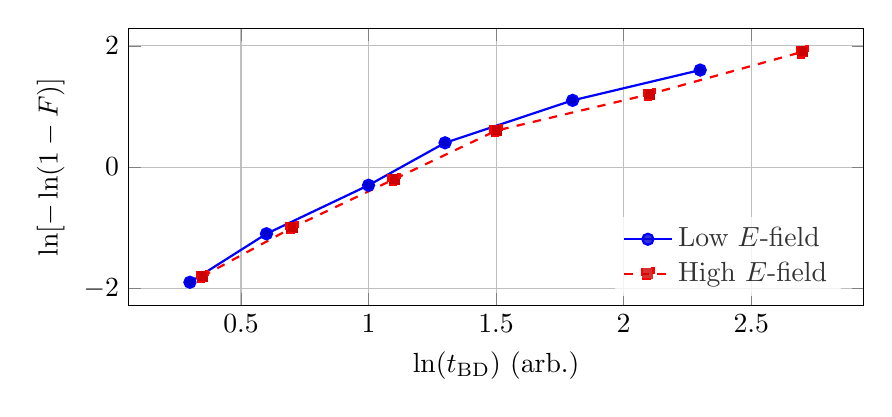
\begin{tikzpicture}
\begin{axis}[
  width=0.9\linewidth,height=0.42\linewidth,
  xlabel={$ \ln(t_{\mathrm{BD}})$ (arb.)},
  ylabel={$ \ln[-\ln(1-F)]$},
  grid=both,
  legend style={at={(0.97,0.03)},anchor=south east,draw=none,fill=white,fill opacity=0.8},
  legend cell align=left]
\addplot+[mark=*,thick] coordinates {(0.30,-1.9) (0.60,-1.1) (1.00,-0.3) (1.30,0.4) (1.80,1.1) (2.30,1.6)};
\addlegendentry{Low $E$-field}
\addplot+[mark=square*, dashed,thick] coordinates {(0.35,-1.8) (0.70,-1.0) (1.10,-0.2) (1.50,0.6) (2.10,1.2) (2.70,1.9)};
\addlegendentry{High $E$-field}
\end{axis}
\end{tikzpicture}
\caption{TDDB Weibull representation at two stress fields (illustrative).}
\label{fig:tddb}
\end{figure}

\end{document}
